\documentclass[a4paper,11pt,pdftex,halfparskip,cleardoubleempty]{scrbook}

\raggedbottom

% \usepackage{fancyhdr}

\usepackage[utf8]{inputenc}
\usepackage{wrapfig}
\usepackage[pdftex]{graphicx}
\usepackage{eso-pic}
\usepackage{array}
\usepackage{tabularx}
\usepackage{float}
\usepackage{listings}

\setlength{\tabcolsep}{20pt}
\renewcommand{\arraystretch}{4}

\graphicspath{{img/}}
\newcommand*{\xchapter}{\stepcounter{chapter}\setcounter{section}{0}\addchap}
\renewcommand*{\thesection}{\arabic{section}}

% define medatata
\def\MTitle{High-Level Modeling and Low-Level Adaption of Serverless Function Choreographies}
\def\MAuthor{Benjamin Walch}
\def\MKeywords{Serverless \sep Function Choreography Language}
\def\MOrg{Universit{\"a}t Innsbruck}
\def\MDate{\today}
\def\MInstitution{Department of Computer Science}
\def\MSupervisor{Dr. Shashko Ristov}
\def\MGroup{Distributed and Parallel Systems}

%
% \pagestyle{fancy}
% \fancyhf{}
% \fancyhead[L]{\leftmark}
% \fancyhead[R]{\thepage}
% \fancyfoot[R]{B. Walch}
% \fancyfoot[L]{Fastlane}

\begin{document}

\frontmatter
\pagestyle{empty}

\begin{titlepage}
\rule{0mm}{1mm}

\begin{multicols}{2}[\columnsep2em] 
	\includegraphics[width=6cm]{uibk-logo}
	\columnbreak
	\begin{flushright}
		\Large{\textsf{\MOrg}}
	\end{flushright}
\end{multicols}

\begin{flushright}
	{\large \MInstitution\\}
	{\large \MGroup}
\end{flushright}

\vspace*{1.5cm}

\begin{center}
	{\LARGE\bf \MTitle}
	\vskip 2.25cm
	\Large \textbf{Bachelor Thesis}
	\vskip 2.25cm
	{\Large \MAuthor}
	\vskip 1.5cm
	{\large Supervisor: \MSupervisor}   
	\vfill
	{\large Innsbruck, \MDate}
\end{center}
\AddToShipoutPicture{
	\put(-55,55){
		\parbox[b]{\paperwidth}{
			\hfill \includegraphics[scale=0.35]{uibk-watermark}
		}
	}
}
\end{titlepage} 

\ClearShipoutPicture

\cleardoublepage

\section*{Declaration}

By  my  own  signature  I  declare  that  I  produced  this  work  as  the  sole author, working independently, and that I did not use any sources and aids other than those referenced in the text. All passages borrowed from external sources, verbatim or by content, are explicitly identified as such.

I consent to the archiving of the bachelor thesis at the institute / faculty:

\vspace{1.8cm}

\parbox{6cm}{
	\hrule
	\strut \centering\footnotesize Date
} \hfill
\parbox{6cm}{
	\hrule
	\strut \centering\footnotesize Signature
}

\cleardoublepage

\pagenumbering{arabic}
\pagestyle{plain}

\section*{Abstract}
"Run code, not Server" is the most recent term of cloud computing providers.
With the rise of the serverless technology during the last years, \emph{FaaS} became more and more popular.
The Distributed and Parallel Systems Group from University of Innsbruck are doing research in this topic.
One of the results of this research is the (generic) specification of the "Abstract Function Choreography Language" (AFCL). Also, a Java API, to describe serverless application workflows programmatically.
The product which results in using that API is the workflow being described in AFCL in a generated YAML or JSON file.
This (textual) workflow definition can then be further processed by (other) machines.
% workflows are abstract
% AFCL

The aim of this bachelor project is to develop a visual workflow editor, which makes modeling of workflows possible at a high level of abstraction. Additionally, composed workflows can be saved, reopened and edited. The tool should also be able to optimize  given workflows for multiple \emph{FaaS} provider(s) in case of quotas and limits, and also in case of performance.

\cleardoublepage

\tableofcontents

\newpage

\section{Introduction}

With the rise of \emph{FaaS}, a high level of flexibility in execution of code appeared. Global Players like Amazon, Google, IBM and Microsoft jumped on the train and provide their infrastructure to Developers, able to deploy functions and execute them in the cloud. Each system has its own definitions on how to define, deploy, run and execute code. 

\label{sec:introduction}
\subsection{Motivation}

\section{Background}

\subsection{FaaS}
\subsection{AFCL}

\section{Overview}

\section{Implementation}
The Implementation of a Graphical User Interface as well as the optimization for Workflows were the main goals of this bachelor thesis. 

\subsection{Requirements}

\begin{itemize}
	\item design for the overall application [coreUI]
	\item clean and intuitive UI [bootstrap]
	\item ability to add components/menu points easily [modularity]
	\item good user experience [SPA]
	\item frameworks: open source, large community (future-safe)
	\item cross-browser [?]
	\item performance [?]
\end{itemize}

\subsection{Frontend}

One of the main parts of the application is the frontend. Since a web based frontend which, runs in the user's web browser, is a hard requirement, the core technologies are limited to HTML, CSS and JavaScript. Before the implementation - in a prototyping phase - different frameworks and libraries have been researched, tested and selected. For the selection, the following criteria have been taken into account:
\begin{itemize}
	\item open-source
	\item good documentation
	\item large and active community (future-proof)
	\item stars on github / downloads on npmtrends
	\item performance
	\item learning curve
\end{itemize}
This criteria ensure the usage of well-documented and open-source software and makes it easier for others (dps) to extend the application later.
The result of this phase was a working prototype as proof-of-concept.
In the following sections, the setup and each technology and corresponding frameworks are described in detail.

% add definitions here (EcmaScript JavaScript

% \subsubsection{Development Workflow}
\subsubsection{Setup}

The setup of the frontend application is a selection of tools and technologies for modern and complex web development.
Under the hood, JavaScript and several JavaScript Frameworks are in action to control the application with all its UI components. To give the application its look and feel, CSS and some CSS Frameworks are in use.
As a basis, Node.js' package manager, npm, is used to manage and resolve the dependencies. Additionally, npm's CLI is used as tool to execute development and/or build tasks. \\
Webpack does much of heavy-lifting, by bundling all sources with the assets into single files, and execute additional build steps by utilizing so-called 'loaders'.
Babel is used as such a webpack loader, for compiling the ECMAScript and React JSX source code to browser-compatible JavaScript.
The same applies for the CSS extension SASS, which is also integrated as a webpack loader, and is used to make the process of styling the user interface more efficient.

\begin{figure}[htbp]
  \centering
  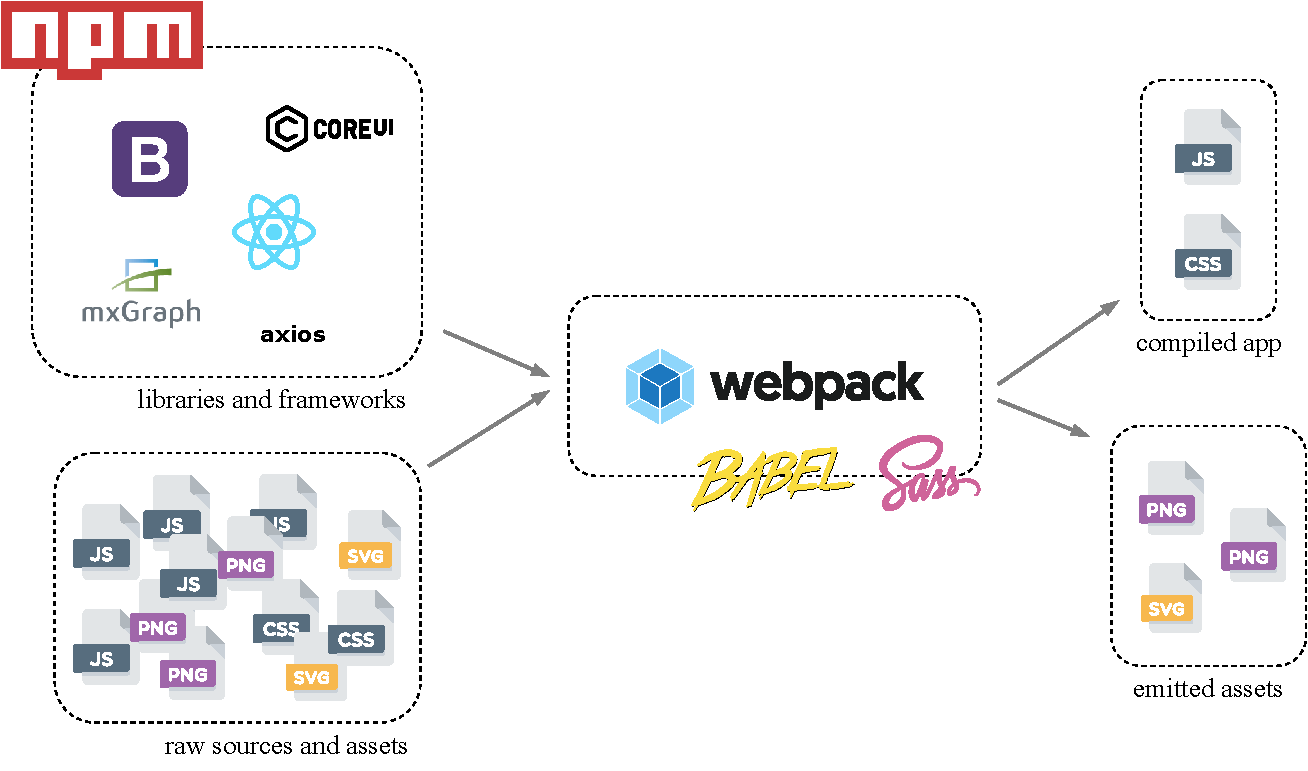
\includegraphics[trim={0.8cm 8.2cm 3.0cm 1cm},scale=0.6]{frontend-setup}
  \caption{frontend development workflow}
\end{figure}
%%% TECHNOLOGIES / TOOLS %%%

\subsubsection{npm}

The node package manager\footnote{https://www.npmjs.org} is the world's largest software registry, where open-source software packages of developers and companies are shared all over the world. Over the last years, npm became a de-facto standard for package management in JavaScript development.

\subsubsection{webpack}

webpack is a module bundler, its main purpose is to bundle JavaScript code for the usage in a browser.\footnote{https://webpack.js.org} In particular, multiple modules (often hundreds of) with dependencies [to each other] are processed and bundled into a few files. To be able to process other types of files than JavaScript or JSON, webpack offers the opportunity to configure a \textbf{loader}. In this application, the following loaders are configured:
\begin{itemize}
\item babel-loader, to transform ECMAScript and React JSX to browser-compatible JavaScript
\item sass-loader, to transform SASS to CSS
\item css-loader, to transform CSS to CommonJS
\item file-loader, to handle static resources like images and fonts
\end{itemize}

\subsubsection{ECMAScript}

The scripting language specification ECMAScript (ES) was created to standardize JavaScript. With the release of ES6 (also known as ECMAScript 2015), features like class declarations, module imports and arrow function expressions became possible. After ES6, every year a new edition of the ECMAScript standard was finalized and released, offering new features. Worth mentioning here is the rest/spread operator released with ES9, which occurs a lot in the source code of this thesis.\\
% spread operator is a lot in use in source code
Since current browsers only have partial support of ECMAScript, a compile 'transcompiler' (or transpiler) is needed to transform the ECMAScript source code to JavaScript common browsers are capable of interpreting.
This process of compiling is done with Babel\footnote{https://babeljs.io}, which is configured to not only compile ECMAScript, but also JSX to JavaScript.

\subsubsection{SASS}

CSS, in its pure form, reaches its limits when one thinks about using variables, functions or nested rules. SASS\footnote{https://sass-lang.com} is a stylesheet language, which is compiled to CSS and offers the mentioned and even more features.
A lot of CSS Frameworks also offer its source code in SASS with a large variable set which makes it easy to customize.

%%% FRAMEWORKS %%%

\subsection{Web Interface}

The layout of the web interface is based on coreUI\footnote{https://coreui.io}, a admin panel template, built on top of the web toolkit Bootstrap\footnote{https://getbootstrap.com}. A clean and nested structure of components, which is typical for a React app, guarantees modularity and forms the whole application. The main component has four sub-components - where each of them consists again of multiple sub-components represent the core features of the app.

\subsubsection{Dashboard}

The dashboard is the entry point where the user lands after accessing the app. The purpose of this component is to give the user a quick overview of the application, provide short informational texts and links to the specific modules. 

\begin{figure}[ht]
  \centering
  \includegraphics[width=\textwidth]{dashboard}
  \caption{the dashboard}
\end{figure}

\subsubsection{Functions}

\begin{figure}[ht]
  \centering
  \includegraphics[width=\textwidth]{functions}
  \caption{the function repository}
\end{figure}

\subsubsection{Editor}

The interface of the workflow compose component is divided in two parts, on the left side the editor and on the right side the property view. The user can choose a function from the toolbar to place it in the drawing area below. Each function has a defined shape and style, for the sake of clarity. These shapes (functions) can then be connected to each other with drag and drop. The possible connection points (ports) of a shape will be displayed when hovering over it. These ports are input and output for most of the functions.\\
When selecting a shape in the canvas, the property view changes. It displays each specific property of the selected function, with the ability to change, add or remove properties.

% Validation

\subsubsection{Settings}


\subsubsection{React}
\subsubsection{mxGraph}
\subsubsection{CoreUI}
\subsubsection{Bootstrap}

%% UI
%% Routing
%% React and Components
%% mxGraph and User Objects

\subsection{Backend}

\subsubsection{General}
\subsubsection{Maven}
\subsubsection{Servlets}
\subsubsection{Api}


\subsection{Continuous Delivery}

\section{Improvements}

\section{Conclusion}


% causes to print all bibliography
\nocite{*}

\bibliographystyle{IEEEtran}
\bibliography{thesis.bib}

\end{document} 
